% Chapter Template

\chapter{Theoretical overview} % Main chapter title

\label{Chapter2} % Change X to a consecutive number; for referencing this chapter elsewhere, use \ref{ChapterX}

\lhead{Chapter 2. \emph{Theoretical overview}} % Change X to a consecutive number; this is for the header on each page - perhaps a shortened title

%----------------------------------------------------------------------------------------
%	SECTION 1
%----------------------------------------------------------------------------------------

\section{Standard model overview}



%-----------------------------------
%	SUBSECTION 1.2
%-----------------------------------
\subsection{Elementary particles of Standard model}

\subsubsection{b quarks}

\subsubsection{Discovery and role of W boson}


%-----------------------------------
%	SUBSECTION 1.2
%-----------------------------------
\subsection{Electroweak interactions}



%-----------------------------------
%	SUBSECTION 1.3
%-----------------------------------

\subsection{Higgs mechanism}


%----------------------------------------------------------------------------------------
%	SECTION 2
%----------------------------------------------------------------------------------------

\section{Wbb at hadron collider}

%-----------------------------------
%	SUBSECTION 2.1
%-----------------------------------

\subsection{Cross sections at hadron colliders}

\begin{figure}[htbp]
	\centering
		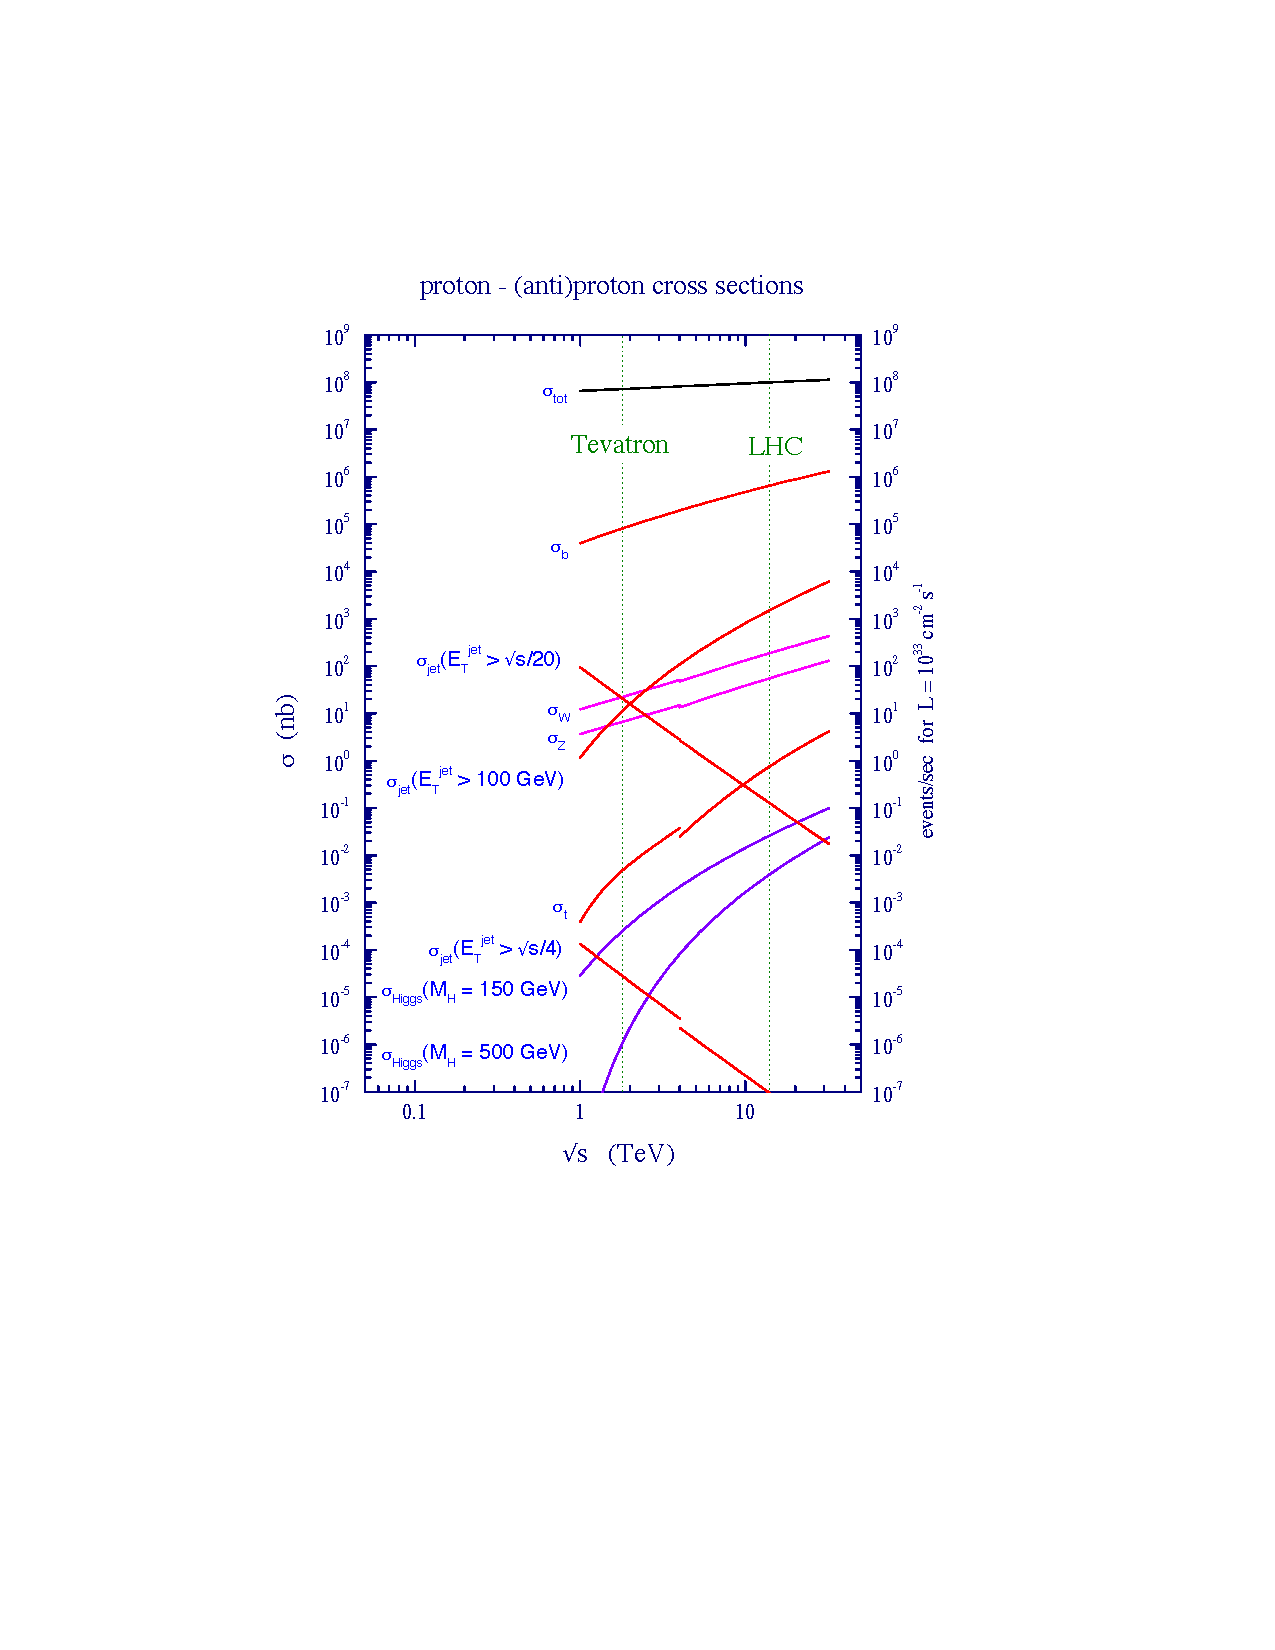
\includegraphics{Figures/pp_xsec.pdf}
		\rule{35em}{0.5pt}
	\caption[Proton-proton cross sections]{Standard model cross sections as a function of center of mass energy.\citep{Campbell:2006wx} }
	\label{fig:pp_xsec}
\end{figure}

%-----------------------------------
%	SUBSECTION 2.2
%-----------------------------------

\subsection{Contributions to Wbb cross section}



%----------------------------------------------------------------------------------------
%	SECTION 3
%----------------------------------------------------------------------------------------

\section{Previous measurements}